\documentclass{beamer}
 
\usepackage[utf8]{inputenc}
\usepackage{graphicx}
\usepackage[font={footnotesize}]{caption}
\usepackage{textcomp}
\usepackage{booktabs}
\usepackage{listings}
\lstset{language=C++,basicstyle=\footnotesize\ttfamily,keywordstyle=\color{red}}
\newcommand{\textapprox}{\raisebox{0.5ex}{\texttildelow}}
\setcounter{tocdepth}{2}
\setbeamertemplate{navigation symbols}{}
\usetheme{Luebeck}

\newcommand\pro{\item[$+$]}
\newcommand\con{\item[$-$]}
%-------------------------------------------------------
%	TITLE PAGE
%-------------------------------------------------------
\title[Geant4-GPU (McMaster University)]{Running Geant4 Functions on a GPU}
\subtitle{Discussion of Results}
\institute{McMaster University}
\author[S. Douglas, R. Gorrie, M .Pagnan, V. Reginato]{
Stuart Douglas -- dougls2
\\Rob Gorrie -- gorrierw
\\Matthew Pagnan -- pagnanmm
\\Victor Reginato -- reginavp
}
 
\begin{document}

\frame{\titlepage}
\begin{frame}
\frametitle{Overview}
\tableofcontents
\end{frame}

% =================== Section =================== 
\section{Introduction} 

\subsection{Brief Project Overview}
\begin{frame}
\frametitle{Brief Project Overview}
Take an existing particle simulation toolkit - Geant4 - and have some functions run on a GPU device to improve performance
\end{frame}

\subsection{Explanation of Terms}
\begin{frame}
\frametitle{What is Geant4?}
\begin{itemize}
\item Geant4 is a toolkit that is meant to simulate the passage of particles through matter
\item It has been developed over the years through collaborative effort of many different institutions and individuals
\item Geant4's diverse particle simulation library has a wide variety of applications including:
\begin{itemize}
\item High energy physics simulations
\item Space and radiation simulations
\item Medical physics simulations
\end{itemize}
\end{itemize}
\end{frame}

\begin{frame}
\frametitle{Demonstration}
\begin{center}
\emph{Demonstration -- Running Geant4 on the CPU}

\emph{Hadr04 With Visualization}
\end{center}
\end{frame}

\begin{frame}
\begin{itemize}
\frametitle{What is GP-GPU Computing?}
\item General-purpose graphic-processing-unit computing is a re-purposing of graphics hardware
\item Allows GPUs  to perform computations that would typically be computed on the CPU
\item If a particular problem is well suited to parallelization, GP-GPU computing can greatly increase performance
\end{itemize}
\end{frame}

\subsection{Scope}
\begin{frame}
\begin{itemize}
\frametitle{Scope}
\item Make current CPU methods available for use on GPU
\begin{itemize}
\item Update build system to support compiling and linking with GPU code
\item Rewrite algorithms in parallel fashion to run on GPU
\end{itemize}
\item Ensure correctness of each GPU-available method by matching results to the corresponding CPU method
\item Compare performance of GPU-available methods to CPU methods
\end{itemize}
\end{frame}

\begin{frame}
\frametitle{Design Phase -- Possible Implementations}
There were initially two different implementation approaches:
\begin{itemize}
\item Port much of Geant4 to the GPU such that each particle runs in parallel
\begin{itemize}
\item Unreasonable given schedule/resource limitations
\end{itemize}
\item Port all methods in some modules to the GPU, storing all relevant data in GPU memory
\begin{itemize}
\item Easy to switch between CPU \& GPU implementations
\item Supports splitting up work by module and by method, and working incrementally
\end{itemize}
\end{itemize}
\end{frame}

\subsection{Purpose}
\begin{frame}
\begin{itemize}
\item Determine if target methods are suitable to parallelization 
\item Increase performance of methods when run on GPU
\item Decrease time required to run simulations involving ported methods
\end{itemize}
\frametitle{Purpose}
\end{frame}

% =================== Section =================== 
\section{Features}
\begin{frame}
\frametitle{Features}
Overview of Main Features:
\begin{itemize}
\item GPU acceleration available on an ``opt-in'' basis
\item Easy to enable/disable GPU acceleration
\item If GPU acceleration is enabled, some methods will run on GPU
\item Same results whether acceleration enabled or disabled
\end{itemize}
\end{frame}

\subsection{Easily Enable/Disable GPU Acceleration}
\begin{frame}
\frametitle{Easily Enable/Disable GPU Acceleration}
\begin{itemize}
\item Existing projects can use GPU acceleration without having to change any code 
\item Flag during build phase enables/disables GPU acceleration
\item Interface remains the same\footnote{implementation 1 only}, acceleration happens behind the scenes
\end{itemize}
\end{frame}

\begin{frame}
\frametitle{Demonstration}
\begin{center}
\emph{Demonstration -- Enabling CUDA Acceleration}
\end{center}
\end{frame}

\begin{frame}[fragile]
\frametitle{Easily Enable/Disable GPU Acceleration}
Methods with GPU versions forwarded to GPU-based implementation at compile time

\begin{block}{Example of Forwarding Method Calls}
\begin{lstlisting}
inline G4double GetY(G4double x)
{
  #if GEANT4_ENABLE_CUDA
    return cudaVector->GetXsec(x);
  #else
    return GetXsec(x);
  #endif
}
\end{lstlisting}
\end{block}
\end{frame}

\begin{frame}
\frametitle{Accelerating Module on GPU}
Existing module \texttt{G4ParticleHPVector} ported to GPU using CUDA\\~\\

\begin{block}{Definition: CUDA}
CUDA is a GP-GPU programming model developed by NVIDIA, for use with NVIDIA graphics cards
\end{block}
\end{frame}

\begin{frame}
\frametitle{\texttt{G4ParticleHPVector} Overview}
Represents empirically-found probabilities of collisions for different particles based on their energy

\begin{itemize}
\item Identified as starting point by relevant stakeholders
\begin{itemize}
\item Used heavily in simulations run by stakeholders
\end{itemize}
\item Seems well-suited to parallelization
\begin{itemize}
\item Based on large vector of 2D points
\item Performs calculations over this vector
\item Sorted by x-value (particle energy)
\end{itemize}
\end{itemize}
\end{frame}

\begin{frame}
\frametitle{Two Implementations}
\begin{enumerate}
\item Forward all calls to existing \texttt{G4ParticleHPVector} interface to a GPU-based implementation of the module

\begin{itemize}
\item Store data vector in GPU memory
\item Copy results back to the CPU to return to the caller
\end{itemize}

\item Add new methods to \texttt{G4ParticleHPVector} interface that are well-suited to GPU computing
\begin{itemize}
\item Copy data vector to GPU memory on method call
\item Existing \texttt{G4ParticleHPVector} methods unchanged, continue to run on CPU
\end{itemize}
\end{enumerate}
\end{frame}

\subsection{Impl. 1: Existing Module in GPU Memory}
\begin{frame}
\frametitle{Impl. 1: Existing Module in GPU Memory}
Calls to \texttt{G4ParticleHPVector} forwarded to new GPU-based class\\~\\

\textbf{Pros:}
\begin{itemize}
\pro Do not have to maintain a copy of the vector on the CPU\footnote{CPU cache was implemented later}
\pro Data rarely copied to GPU memory
\end{itemize}
\textbf{Cons:}
\begin{itemize}
\con All methods are run on the GPU, even if not well-suited to parallelism
\con Return values must be copied from GPU memory to CPU memory (slow)
\end{itemize}
\end{frame}

\begin{frame}
\frametitle{Demonstration}
\begin{center}
\emph{Demonstration -- Running Geant4 on the GPU}

\emph{Hadr04 With Visualization}

\end{center}
\end{frame}

\begin{frame}[fragile]
\frametitle{Caching Data Vector in CPU Memory}
To improve data-copying performance, maintain cache of data in CPU memory as well
\begin{itemize}
\item Only updated when necessary
\item For methods that are not parallelizable, can run on CPU using cached data
\end{itemize}
\begin{block}{CopyToCpuIfDirty}
\begin{lstlisting}
if (isDataDirtyHost) {
   cudaMemcpy(h_theData, d_theData, nEntries);
   isDataDirtyHost = false;
}
\end{lstlisting}
\end{block}

\end{frame}

\subsubsection{Implementation of Select Methods on GPU}
\begin{frame}[fragile]
\frametitle{Impl. 1 -- \texttt{Times}}
Multiplies each element in data vector by factor
\begin{block}{Times\_CUDA}
\begin{lstlisting} 
int tid = blockDim.x * blockIdx.x + threadIdx.x;
if (tid < nEntries) 
   theData[tid].xSec = theData[tid].xSec * factor;    
\end{lstlisting}
\end{block}
\end{frame}

\begin{frame}[fragile]
\frametitle{Impl. 1 -- \texttt{GetXSec}}
Returns y-value of first point with energy at least \texttt{e} parameter
\begin{block}{GetXSec\_CUDA}
\begin{lstlisting}
int start = blockDim.x * blockIdx.x + threadIdx.x;
for (int i = start; i < nEntries; i += numThreads)
   if (theData[i].energy >= e) {
      resultIndex = Min(resultIndex, i);
      return;
    }
\end{lstlisting}
\end{block}
\end{frame}

\subsubsection{Impl. 1: Performance}
\begin{frame}
\frametitle{Impl. 1: Performance Results Summary}
\begin{itemize}
\item Methods generally slower on GPU until \textapprox 10,000 entries in data vector
\item Most \emph{commonly-used} methods significantly slower on GPU, even with large data vector
\begin{itemize}
\item Lots of data copying
\end{itemize}
\item Many problems in vector class not well-suited to parallelism
\end{itemize}
\end{frame}

\begin{frame}
\frametitle{Impl. 1: Performance Results -- \texttt{Times}}
Multiplies each point in vector by factor
\begin{figure}
\centering
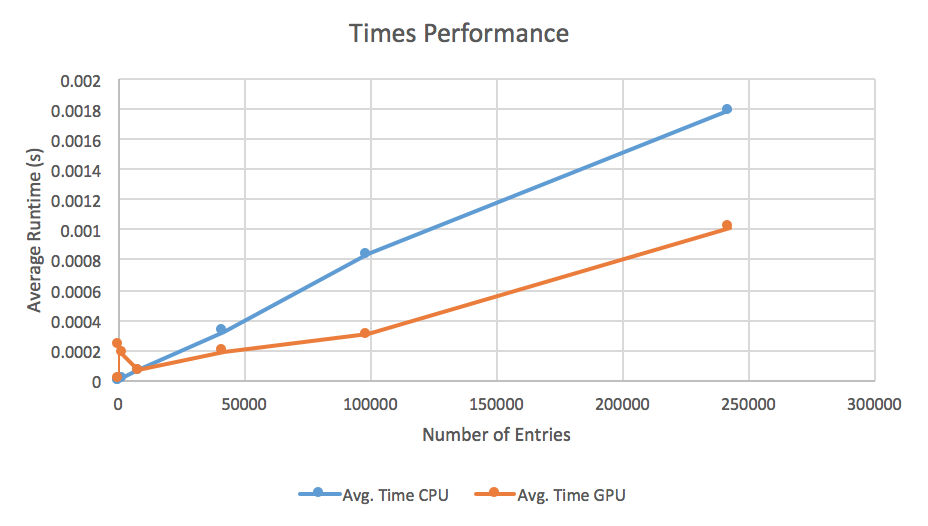
\includegraphics[width=0.8\textwidth]{images/times_line.png}
\caption{Runtime vs. Number of Data Points -- \texttt{Times}}
\end{figure}
\end{frame}

\begin{frame}
\frametitle{Impl. 1: Performance Results -- \texttt{GetXSec}}
Returns y-value of first point with energy at least `\texttt{e}'
\begin{figure}
\centering
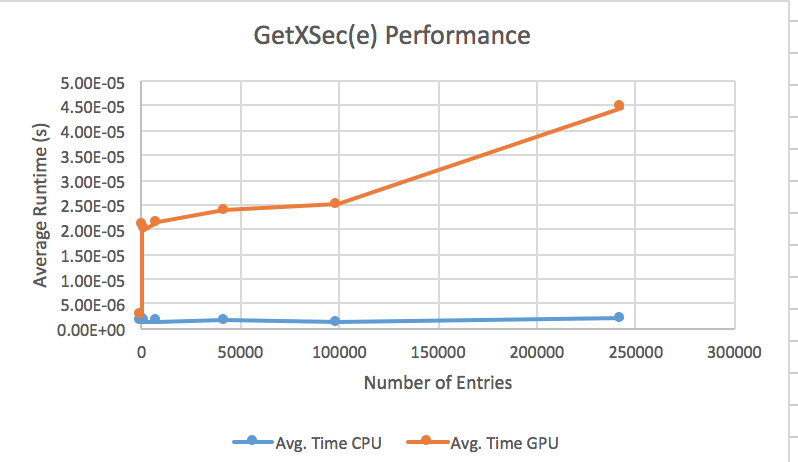
\includegraphics[width=0.8\textwidth]{images/getxsec_e_line.png}
\caption{Runtime vs. Number of Data Points -- \texttt{GetXSec}}
\end{figure}
\end{frame}

\begin{frame}
\frametitle{Impl. 1: Performance Results -- \texttt{SampleLin}}
Interpolates between two random, consecutive points and their corresponding integrals
\begin{figure}
\centering
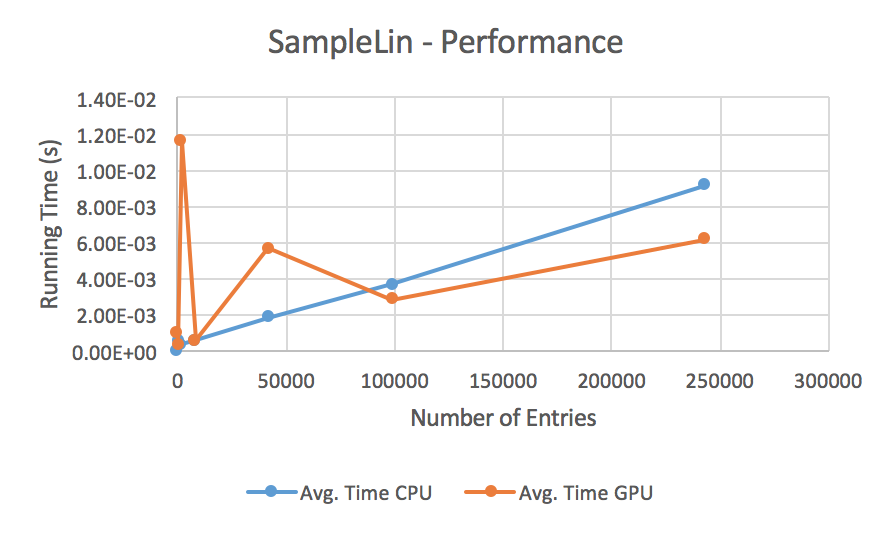
\includegraphics[width=0.8\textwidth]{images/samplelin_line.png}
\caption{Runtime vs. Number of Data Points -- \texttt{SampleLin}}
\end{figure}
\end{frame}

\begin{frame}
\frametitle{Impl. 1: Performance Results -- System Tests}
System Test \#1:
\begin{table}
	\begin{tabular}{lll}
	\toprule
	\bf CPU Time&\bf  GPU Time&\bf Speedup of GPU\\\midrule
	54.55s&72.08s&-1.32$\times$\\\bottomrule
	\end{tabular}
	\caption{Performance - Water, 500 events}
\end{table}
System Test \#2:
\begin{table}
	\begin{tabular}{lll}
	\toprule
	\bf CPU Time&\bf  GPU Time&\bf Speedup of GPU\\\midrule
	54.55s&72.08s&-1.32$\times$\\\bottomrule
	\end{tabular}
	\caption{Performance - Water, 2000 events}
\end{table}
\end{frame}

\begin{frame}
\frametitle{Impl. 1: Performance Discussion}
\begin{itemize}
\item Simple ``getters'' and ``setters'' now require copy from GPU to CPU memory
\item Current code calling \texttt{G4ParticleHPVector} more data-oriented than computation-oriented
\item Low \texttt{GetXSec} performance due to lack of \texttt{Hash} object on GPU to accelerate finding min index
\item Although some methods faster, rarely used in practice
\end{itemize}
\end{frame}

\subsection{Impl. 2: Add New GPU-Accelerated Methods to Interface}
\begin{frame}
\frametitle{Impl. 2: Add New GPU-Accelerated Methods to Interface}
Add new methods to \texttt{G4ParticleHPVector} interface that are well-suited to parallelism\\~\\

\textbf{Pros:}
\begin{itemize}
\pro Only methods that run faster on the GPU are implemented
\end{itemize}

\textbf{Cons:}
\begin{itemize}
\con Will have to maintain two copies of the data vector
\con Will need to copy the vector to the GPU whenever method called
\end{itemize}
\end{frame}

\begin{frame}
\frametitle{Impl. 2: \texttt{GetXSecList}}
\texttt{GetXSecList} Overview
\begin{itemize}
\item Fill an array of energies for which we want the cross section values for
\item Send the array to the GPU to work on
\item Each thread works on its own query(s)
\end{itemize}
\end{frame}

\begin{frame}[fragile]
\frametitle{Implementation -- \texttt{GetXSecList}}
\begin{block}{GetXSecList}
\begin{lstlisting}[language=C++,basicstyle=\ttfamily,keywordstyle=\color{red}]
stepSize = sqrt(nEntries);
e = queryList[threadID];
    
for (int i = 0; i < nEntries; i += stepSize) 
   if (d_theData[i].energy >= e) 
      break;
\end{lstlisting}
\end{block}
\end{frame}

\begin{frame}[fragile]
\frametitle{Implementation -- \texttt{GetXSecList} Cont.}
\begin{block}{GetXSecList -- cont}
\begin{lstlisting}[language=C++, basicstyle=\ttfamily, keywordstyle=\color{red}]
i =  i - (stepSize - 1); 

for (; i < nEntries; i++) 
   if (d_theData[i].energy >= e) 
      break;
   
d_queryList[threadID] = i;
\end{lstlisting}
\end{block}
\end{frame}


\subsubsection{Impl. 2: Performance}
\begin{frame}
\frametitle{Impl. 2: Performance Results Summary}
Performance of implementation 2 also proved slower than 
similar CPU-based method
\begin{itemize}
\item Performance on GPU linear to number of elements in data array
\item Performance on CPU not affected by number of elements after point, due to saved hashes
\end{itemize}
\end{frame}

\begin{frame}
\frametitle{Impl. 2: Performance Results -- \texttt{GetXSecList}}
\begin{figure}
\centering
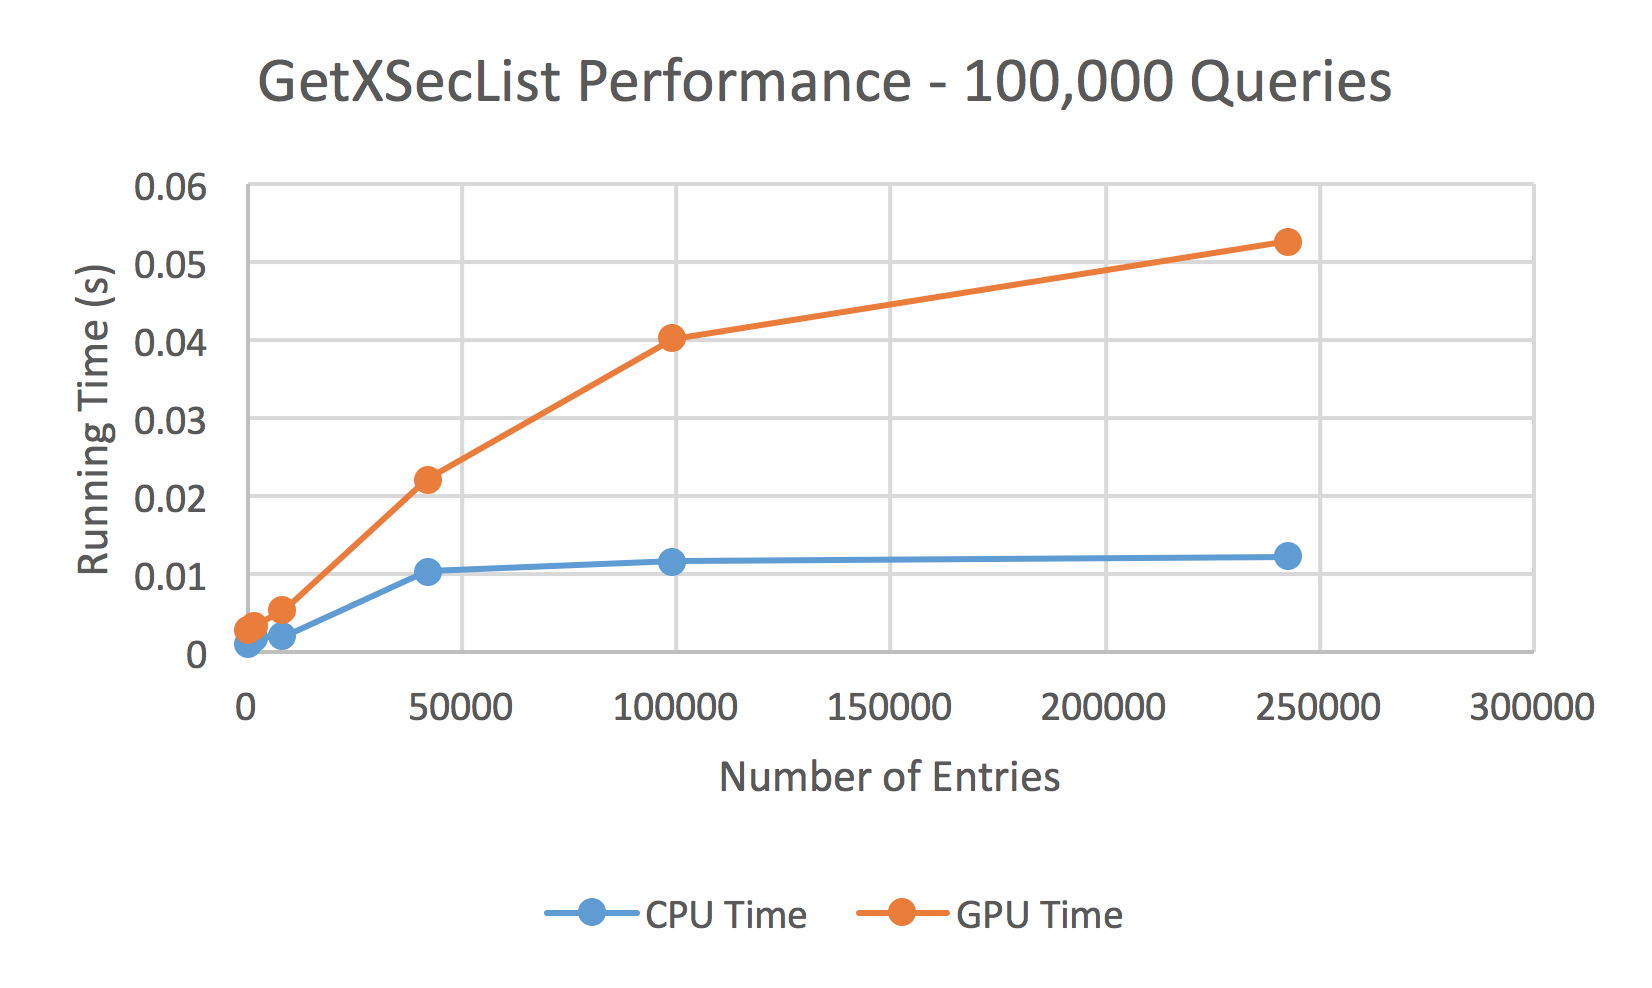
\includegraphics[width=0.8\textwidth]{images/getxseclist_100000.png}
\caption{Runtime vs. Number of Data Points -- \texttt{GetXSecList}, 100,000 Queries}
\end{figure}
\end{frame}

\begin{frame}
\frametitle{Impl. 2: Performance Discussion}
\begin{itemize}
\item CPU implementation makes use of \texttt{Hash} to quickly find minimum index
\item Finding first element satisfying predicate not well-suited to parallelism
\item If one thread finds element, must wait for all other threads (blocking divergence)
\end{itemize}
\end{frame}

\subsection{Accuracy / Testing}
\begin{frame}
\frametitle{Accuracy}
\begin{itemize}
\item All modified methods except \texttt{SampleLin} and \texttt{Sample}
yield results that precisely match original implementations
\begin{itemize}
\item Some methods fell extremely close in accuracy to 
the original, and were considered to `pass'
\item For \texttt{Sample} and \texttt{SampleLin}, the average of 1000 tests was compared, with a relative error tolerance of 0.01
\end{itemize}

\item The system test results differ with more than 500 events
\begin{itemize}
\item \texttt{Sample} and \texttt{SampleLin} only called if more than 500 events
\end{itemize}
\end{itemize}
\end{frame}

\begin{frame}
\frametitle{Accuracy Discussion}
\begin{itemize}
\item The deviations in \texttt{SampleLin} and \texttt{Sample} can be 
attributed to their use of random numbers
\begin{itemize}
\item CUDA random number generator will have different results than \texttt{rand()}
\item Both methods take random point and interpolate it and its neighbour, so values differ significantly based on random number
\end{itemize}
\item The negligible deviations in other ported methods 
are attributed to small differences in CPU and GPU 
arithmetic round-off errors (\texttt{log}, \texttt{exp}, etc.)
\end{itemize}
\end{frame}

\begin{frame}
\frametitle{Testing}
\begin{itemize}
\item Comparing test results and performance with GPU acceleration enabled and disabled
\item Testing framework based on two phases, one program for each phase
\begin{enumerate}
\item \texttt{GenerateTestResults:} Run unit tests and save results to file
\item \texttt{AnalyzeTestResults:} Compare results from CPU and GPU
\end{enumerate}
\item Run \texttt{GenerateTestResults} once with GPU acceleration enabled, once with it disabled
\end{itemize}
\end{frame}

\begin{frame}[fragile]
\frametitle{\texttt{GenerateTestResults} Details}
\begin{itemize}
\item Outputs simple results directly to results file
\item For arrays, calculates hash for array and output it
\item Outputs timing data to separate file
\end{itemize}
\begin{block}{Example: Snippet of Generated Test Results}
\begin{lstlisting}
#void G4ParticleHPVector_CUDA::GetXsecBuffer(
  G4double * queryList, G4int length)_6
@numQueries=10
hash: 16548307878283220284
@numQueries=50
hash: 3204132713354913775
\end{lstlisting}
\end{block}
\end{frame}

\begin{frame}
\frametitle{\texttt{AnalyzeTestResults} Details}
Two main functions:
\begin{enumerate}
\item Compare results for each test case, printing status to \texttt{stdout}
\begin{itemize}
\item If test failed, output differing values
\item Summarize test results at the end
\end{itemize}
\item Generate \texttt{.csv} file from timing data
\begin{itemize}
\item One row per unique method call comparing CPU and GPU times
\item Can use Excel to analyze performance results
\end{itemize}
\end{enumerate}
\end{frame}

\begin{frame}
\frametitle{Demonstration}
\begin{center}
\emph{Demonstration -- Analyzing Test Results}
\end{center}
\end{frame}

\section{Conclusion}
\subsection{Summary of Results}
\begin{frame}
\frametitle{Summary of Results}
\begin{itemize}
\item Impl. 1 was about 1.3X slower on average in system tests
\item Impl. 2 was about 4X slower in unit tests
\item Most commonly-used methods not well-suited to parallelism
\item \texttt{Sample} and \texttt{SampleLin} have accuracy issues due to random number generation
\end{itemize}
\end{frame}

\subsection{Recommendations}
\begin{frame}
For further work parallelizing Geant4:
\begin{itemize}
\item Use Geant4-GPU project as framework for parallelizing other modules
\item Look for modules storing large amounts of structured data
\item Methods with nested loops are prime candidates for parallelization
\item Probabilistic methods and getter/setter methods won't have considerable benefits
\item Methods with extensive conditional branching may cause difficulties in parallelizing
\end{itemize}
\end{frame}

\subsection{Final Thoughts}
\begin{frame}
\frametitle{Conclusion}
\begin{itemize}
\item All project collaborators have gained a lot of experience
\item Lack of speedup disappointing, but lets us know \texttt{G4ParticleHPVector} not perfect candidate
\item Parallelization of existing software is hard
\end{itemize}
\end{frame}

\end{document}
